\documentclass[border=12pt]{standalone}
\usepackage{xcolor}
\usepackage{tikz}
\usetikzlibrary{arrows.meta,positioning,fit,backgrounds,calc}

% Palette lifted from the discovery pipeline diagram for a consistent look.
\definecolor{INK}{HTML}{1A1A2E}
\definecolor{MUTED}{HTML}{8A8F99}
\definecolor{BG}{HTML}{FAFAFA}
\definecolor{BLUE}{HTML}{4361EE}
\definecolor{BLUEBG}{HTML}{EAEEFD}
\definecolor{GREEN}{HTML}{0B7A4B}
\definecolor{GREENBG}{HTML}{E4F2EB}
\definecolor{PINK}{HTML}{D81159}
\definecolor{PINKBG}{HTML}{FBE6EE}
\definecolor{FOOT}{HTML}{E1E4EA}

\begin{document}
\pagecolor{BG}
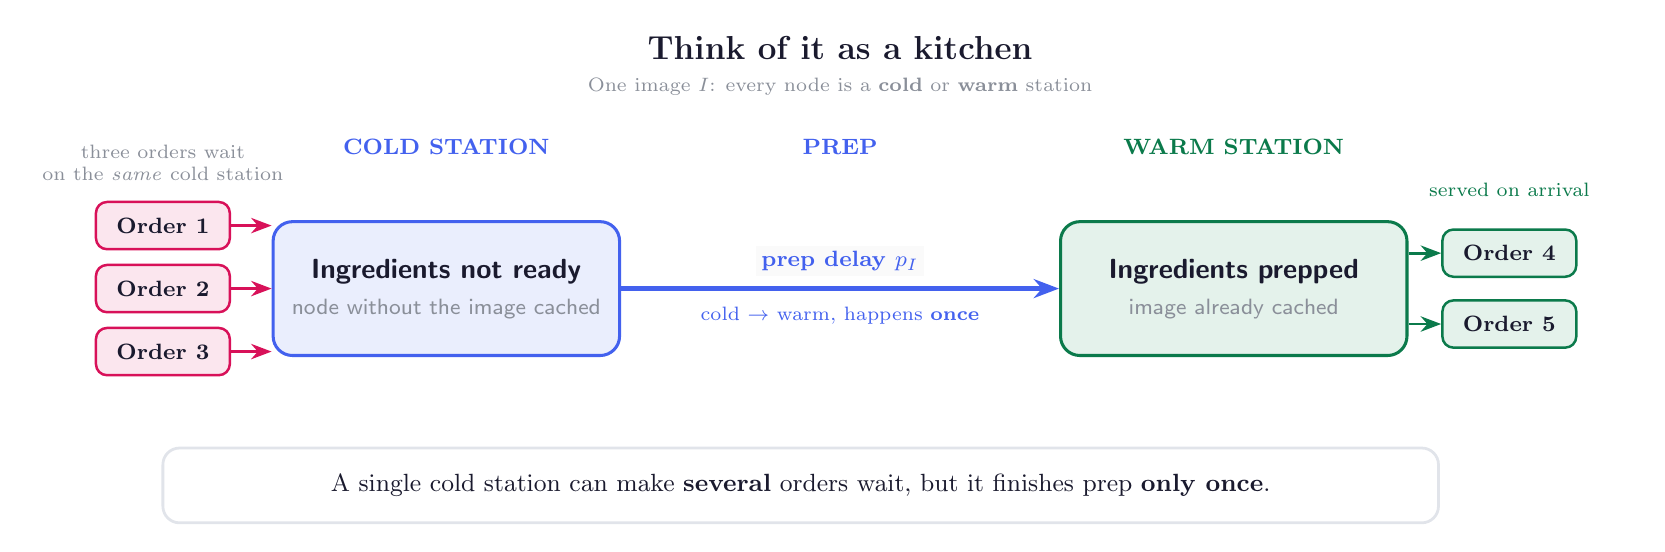
\begin{tikzpicture}[
  font=\sffamily,
  station/.style={rounded corners=7pt, line width=1.1pt, minimum width=4.4cm,
    minimum height=1.7cm, align=center, text=INK},
  cold/.style={station, draw=BLUE, fill=BLUEBG},
  warm/.style={station, draw=GREEN, fill=GREENBG},
  job/.style={rounded corners=4pt, draw=PINK, fill=PINKBG, line width=0.9pt,
    minimum width=1.7cm, minimum height=0.6cm, align=center, text=INK,
    font=\footnotesize\bfseries},
  hdr/.style={font=\footnotesize\bfseries, text=MUTED},
  sub/.style={font=\scriptsize, text=MUTED},
  flow/.style={-{Stealth[length=2.6mm]}, draw=PINK, line width=1.0pt},
  prep/.style={-{Stealth[length=3.2mm]}, draw=BLUE, line width=1.6pt},
]

% ---- title ----------------------------------------------------------------
\node[font=\large\bfseries, text=INK] at (7.6,6.6) {Think of it as a kitchen};
\node[sub] at (7.6,6.12) {One image \(I\): every node is a \textbf{cold} or \textbf{warm} station};

% ---- section headers ------------------------------------------------------
\node[hdr, text=BLUE] at (2.6,5.35) {COLD STATION};
\node[hdr, text=BLUE] at (7.6,5.35) {PREP};
\node[hdr, text=GREEN] at (12.6,5.35) {WARM STATION};

% ---- stations -------------------------------------------------------------
\node[cold] (cold) at (2.6,3.55) {\textbf{Ingredients not ready}\\[1pt]{\footnotesize\color{MUTED}node without the image cached}};
\node[warm] (warm) at (12.6,3.55) {\textbf{Ingredients prepped}\\[1pt]{\footnotesize\color{MUTED}image already cached}};

% ---- orders queued at the cold station ------------------------------------
\node[job] (j1) at (-1.0,4.35) {Order 1};
\node[job] (j2) at (-1.0,3.55) {Order 2};
\node[job] (j3) at (-1.0,2.75) {Order 3};
\draw[flow] (j1.east) -- (cold.west |- j1.east);
\draw[flow] (j2.east) -- (cold.west |- j2.east);
\draw[flow] (j3.east) -- (cold.west |- j3.east);
\node[sub, align=center, text width=3.2cm] at (-1.0,5.15)
  {three orders wait\\on the \emph{same} cold station};

% ---- orders served instantly at the warm station --------------------------
\node[job, draw=GREEN, fill=GREENBG] (j4) at (16.1,4.0) {Order 4};
\node[job, draw=GREEN, fill=GREENBG] (j5) at (16.1,3.1) {Order 5};
\draw[-{Stealth[length=2.6mm]}, draw=GREEN, line width=1.0pt] (warm.east |- j4.west) -- (j4.west);
\draw[-{Stealth[length=2.6mm]}, draw=GREEN, line width=1.0pt] (warm.east |- j5.west) -- (j5.west);
\node[sub, align=center, text width=3.0cm, text=GREEN] at (16.1,4.8)
  {served on arrival};

% ---- prep-delay arrow (cold -> warm) --------------------------------------
\draw[prep] (cold.east) -- (warm.west);
\node[font=\footnotesize\bfseries, text=BLUE, fill=BG, inner sep=2pt] at (7.6,3.9) {prep delay \(p_I\)};
\node[sub, text=BLUE] at (7.6,3.2) {cold \(\rightarrow\) warm, happens \textbf{once}};

% ---- footer bar -----------------------------------------------------------
\node[rounded corners=6pt, draw=FOOT, fill=white, line width=1.0pt,
  minimum width=16.2cm, minimum height=0.95cm, align=center, text=INK,
  font=\small] (foot) at (7.1,1.05)
  {A single cold station can make \textbf{several} orders wait, but it finishes prep \textbf{only once}.};

\end{tikzpicture}
\end{document}
